% Options for packages loaded elsewhere
\PassOptionsToPackage{unicode}{hyperref}
\PassOptionsToPackage{hyphens}{url}
\PassOptionsToPackage{dvipsnames,svgnames,x11names}{xcolor}
%
\documentclass[
]{article}

\usepackage{amsmath,amssymb}
\usepackage{iftex}
\ifPDFTeX
  \usepackage[T1]{fontenc}
  \usepackage[utf8]{inputenc}
  \usepackage{textcomp} % provide euro and other symbols
\else % if luatex or xetex
  \usepackage{unicode-math}
  \defaultfontfeatures{Scale=MatchLowercase}
  \defaultfontfeatures[\rmfamily]{Ligatures=TeX,Scale=1}
\fi
\usepackage{lmodern}
\ifPDFTeX\else  
    % xetex/luatex font selection
\fi
% Use upquote if available, for straight quotes in verbatim environments
\IfFileExists{upquote.sty}{\usepackage{upquote}}{}
\IfFileExists{microtype.sty}{% use microtype if available
  \usepackage[]{microtype}
  \UseMicrotypeSet[protrusion]{basicmath} % disable protrusion for tt fonts
}{}
\makeatletter
\@ifundefined{KOMAClassName}{% if non-KOMA class
  \IfFileExists{parskip.sty}{%
    \usepackage{parskip}
  }{% else
    \setlength{\parindent}{0pt}
    \setlength{\parskip}{6pt plus 2pt minus 1pt}}
}{% if KOMA class
  \KOMAoptions{parskip=half}}
\makeatother
\usepackage{xcolor}
\setlength{\emergencystretch}{3em} % prevent overfull lines
\setcounter{secnumdepth}{5}
% Make \paragraph and \subparagraph free-standing
\makeatletter
\ifx\paragraph\undefined\else
  \let\oldparagraph\paragraph
  \renewcommand{\paragraph}{
    \@ifstar
      \xxxParagraphStar
      \xxxParagraphNoStar
  }
  \newcommand{\xxxParagraphStar}[1]{\oldparagraph*{#1}\mbox{}}
  \newcommand{\xxxParagraphNoStar}[1]{\oldparagraph{#1}\mbox{}}
\fi
\ifx\subparagraph\undefined\else
  \let\oldsubparagraph\subparagraph
  \renewcommand{\subparagraph}{
    \@ifstar
      \xxxSubParagraphStar
      \xxxSubParagraphNoStar
  }
  \newcommand{\xxxSubParagraphStar}[1]{\oldsubparagraph*{#1}\mbox{}}
  \newcommand{\xxxSubParagraphNoStar}[1]{\oldsubparagraph{#1}\mbox{}}
\fi
\makeatother


\providecommand{\tightlist}{%
  \setlength{\itemsep}{0pt}\setlength{\parskip}{0pt}}\usepackage{longtable,booktabs,array}
\usepackage{calc} % for calculating minipage widths
% Correct order of tables after \paragraph or \subparagraph
\usepackage{etoolbox}
\makeatletter
\patchcmd\longtable{\par}{\if@noskipsec\mbox{}\fi\par}{}{}
\makeatother
% Allow footnotes in longtable head/foot
\IfFileExists{footnotehyper.sty}{\usepackage{footnotehyper}}{\usepackage{footnote}}
\makesavenoteenv{longtable}
\usepackage{graphicx}
\makeatletter
\def\maxwidth{\ifdim\Gin@nat@width>\linewidth\linewidth\else\Gin@nat@width\fi}
\def\maxheight{\ifdim\Gin@nat@height>\textheight\textheight\else\Gin@nat@height\fi}
\makeatother
% Scale images if necessary, so that they will not overflow the page
% margins by default, and it is still possible to overwrite the defaults
% using explicit options in \includegraphics[width, height, ...]{}
\setkeys{Gin}{width=\maxwidth,height=\maxheight,keepaspectratio}
% Set default figure placement to htbp
\makeatletter
\def\fps@figure{htbp}
\makeatother
% definitions for citeproc citations
\NewDocumentCommand\citeproctext{}{}
\NewDocumentCommand\citeproc{mm}{%
  \begingroup\def\citeproctext{#2}\cite{#1}\endgroup}
\makeatletter
 % allow citations to break across lines
 \let\@cite@ofmt\@firstofone
 % avoid brackets around text for \cite:
 \def\@biblabel#1{}
 \def\@cite#1#2{{#1\if@tempswa , #2\fi}}
\makeatother
\newlength{\cslhangindent}
\setlength{\cslhangindent}{1.5em}
\newlength{\csllabelwidth}
\setlength{\csllabelwidth}{3em}
\newenvironment{CSLReferences}[2] % #1 hanging-indent, #2 entry-spacing
 {\begin{list}{}{%
  \setlength{\itemindent}{0pt}
  \setlength{\leftmargin}{0pt}
  \setlength{\parsep}{0pt}
  % turn on hanging indent if param 1 is 1
  \ifodd #1
   \setlength{\leftmargin}{\cslhangindent}
   \setlength{\itemindent}{-1\cslhangindent}
  \fi
  % set entry spacing
  \setlength{\itemsep}{#2\baselineskip}}}
 {\end{list}}
\usepackage{calc}
\newcommand{\CSLBlock}[1]{\hfill\break\parbox[t]{\linewidth}{\strut\ignorespaces#1\strut}}
\newcommand{\CSLLeftMargin}[1]{\parbox[t]{\csllabelwidth}{\strut#1\strut}}
\newcommand{\CSLRightInline}[1]{\parbox[t]{\linewidth - \csllabelwidth}{\strut#1\strut}}
\newcommand{\CSLIndent}[1]{\hspace{\cslhangindent}#1}

\makeatletter
\@ifpackageloaded{caption}{}{\usepackage{caption}}
\AtBeginDocument{%
\ifdefined\contentsname
  \renewcommand*\contentsname{Table of contents}
\else
  \newcommand\contentsname{Table of contents}
\fi
\ifdefined\listfigurename
  \renewcommand*\listfigurename{List of Figures}
\else
  \newcommand\listfigurename{List of Figures}
\fi
\ifdefined\listtablename
  \renewcommand*\listtablename{List of Tables}
\else
  \newcommand\listtablename{List of Tables}
\fi
\ifdefined\figurename
  \renewcommand*\figurename{Figure}
\else
  \newcommand\figurename{Figure}
\fi
\ifdefined\tablename
  \renewcommand*\tablename{Table}
\else
  \newcommand\tablename{Table}
\fi
}
\@ifpackageloaded{float}{}{\usepackage{float}}
\floatstyle{ruled}
\@ifundefined{c@chapter}{\newfloat{codelisting}{h}{lop}}{\newfloat{codelisting}{h}{lop}[chapter]}
\floatname{codelisting}{Listing}
\newcommand*\listoflistings{\listof{codelisting}{List of Listings}}
\makeatother
\makeatletter
\makeatother
\makeatletter
\@ifpackageloaded{caption}{}{\usepackage{caption}}
\@ifpackageloaded{subcaption}{}{\usepackage{subcaption}}
\makeatother

\ifLuaTeX
  \usepackage{selnolig}  % disable illegal ligatures
\fi
\usepackage{bookmark}

\IfFileExists{xurl.sty}{\usepackage{xurl}}{} % add URL line breaks if available
\urlstyle{same} % disable monospaced font for URLs
\hypersetup{
  pdftitle={Unveiling the Complexity of Food Webs: A Comprehensive Overview of Definitions, Scales, and Mechanisms},
  pdfauthor={Tanya Strydom; Jennifer A. Dunne; Timothée Poisot; Andrew P. Beckerman},
  pdfkeywords={food web, network construction, scientific ignorance},
  colorlinks=true,
  linkcolor={blue},
  filecolor={Maroon},
  citecolor={Blue},
  urlcolor={Blue},
  pdfcreator={LaTeX via pandoc}}



\title{Unveiling the Complexity of Food Webs: A Comprehensive Overview
of Definitions, Scales, and Mechanisms}
\author{Tanya Strydom %
%
\textsuperscript{%
%
1%
}%
; Jennifer A. Dunne %
%
\textsuperscript{%
%
2%
}%
; Timothée Poisot %
%
\textsuperscript{%
3,%
4%
}%
; Andrew P. Beckerman %
%
\textsuperscript{%
%
1%
}%
}
\date{2024-09-13}

\usepackage{setspace}
\usepackage[left]{lineno}
\usepackage[letterpaper]{geometry}

\usepackage[nolists,noheads,markers]{endfloat}
\geometry{margin=2.5cm}

\begin{document}

\thispagestyle{empty}
{\bfseries\sffamily\Large Unveiling the Complexity of Food Webs: A
Comprehensive Overview of Definitions, Scales, and Mechanisms}
\vfil
Tanya Strydom %
%
\textsuperscript{%
%
1%
}%
; Jennifer A. Dunne %
%
\textsuperscript{%
%
2%
}%
; Timothée Poisot %
%
\textsuperscript{%
3,%
4%
}%
; Andrew P. Beckerman %
%
\textsuperscript{%
%
1%
}%

\vfil
{\small
\textbf{Abstract:} Food webs are a useful abstraction and representation
of the feeding links between species in a community and are used to
infer many ecosystem level processes. However, the different theories,
mechanisms, and criteria that underpin how a food web is defined and,
ultimately, constructed means that not all food webs are representing
the same ecological process. Here we present a synthesis of the
different assumptions, scales and mechanisms that are used to define
different ecological networks ranging from metawebs (an inventory of all
potential interactions) to fully realised networks (interactions that
occur within a given community over a certain timescale). Illuminating
the assumptions, scales, and mechanisms of network inference allows a
formal categorisation of how to use networks to answer key ecological
and conservation questions and defines guidelines to prevent
unintentional misuse or misinterpretation.
\vfil
\textbf{Keywords:} %
food web, network construction, %
scientific ignorance%
}
\clearpage
\setcounter{page}{1}
\doublespacing
\linenumbers


At the heart of modern biodiversity science are a set of concepts and
theories about biodiversity, stability and function. These relate to the
abundance, distribution and services that biodiversity provides, and how
biodiversity -- as an interconnected set of species -- responds to
multiple stressors. The interaction between species (or individuals) is
one of the fundamental building blocks of ecological communities provide
a powerful abstraction that can help quantify, conceptualise, and
understand biodiversity dynamics, and ultimately, one hopes, make
prediction, mitigate change and manage services {[}ref{]}. Such network
representations of biodiversity (including within species diversity) are
increasingly argued to be an asset to predictive ecology, climate change
mitigation and resource management. Here, it is argued that
characterising biodiversity in a network will allow deeper capacity to
understand and predict the abundance, distribution, dynamics and
services provided by multiple species facing multiple stressors.

However, the way that a network is constructed (encoded) defines an
epistemology of the network concept which, we argue, can influence the
resulting observations and conclusions about pattern and mechanisms that
are made (Brimacombe et al., 2023; Proulx et al., 2005). This process of
constructing networks has two major pillars: the data and theory, the
latter representing an expression of mechanism and process giving rise
to patterns that emerge from collating interactions among species. Each
of these pillars carries with it a set of practical, semantic and
conceptual constraints that not only influence progress in making
network ecology more valuable and potentially predictive, but help
define the spatial, temporal and evolutionary scale of assumptions we
make and predictions we might generate from the networks.

With respect to data, it is extremely challenging to actually record
species interactions in the field (Jordano, 2016a, 2016b). Despite
notable herculean efforts (\textbf{Woodward? Benguela?} Maiorano et al.
(2020)), actual coverage of `real world' interaction data remains sparse
(Poisot et al., 2021). Against this practical challenge, there is
additionally high variance in the terminology we use to define networks.
Finally, the mathematical and statistical tools we use to construct,
conceptualise, analyse and predict with these networks are also highly
variable.

\begin{enumerate}
\def\labelenumi{\arabic{enumi}.}
\tightlist
\item
  what are the underlying assumptions about nodes, edges, scale and
  process that are made when we attempt to delimit and describe a food
  webs;
\item
  are there families of commonly used tools that map onto assumptions
  about scales and processes;
\end{enumerate}

The provision of this detail ultimately leads to a set of insights and
conclusions about whether, when and under what conditions network
representations of biodiversity can contribute to the advancement of
ecological theory and generate value in predictive ecology.
Specifically, we finish this perspective with an overview of fundamental
questions in ecology that we think can benefit from network thinking and
a proposal that such thinking can accelerate our capacity to predict the
impact of multiple stressors on biodiverse communities.

\section{Setting the Scene: The Not So Basics of Nodes and
Edges}\label{sec-anatomy}

Defining a food web seems simple; it is the representation of the
interactions (edges) between species (nodes), however the definition of
`edges' and `nodes', as well as the scale at which they are aggregated
can take many forms (Poisot, Stouffer, et al., 2016). Networks can be
constructed at the population (the links among individuals), community
(the links between species), or metacommunity (changes between
locations) level. Even if one were to limit their scope to thinking of
interaction networks only in terms of food webs at the community-level
there are still many ways to define the various components of the
network Panel A of~\ref{fig-anatomy}, one needs to understand the
different intentions/assumptions that are made when a food web is
constructed. Although the main goal of constructing a food web is to
capture and represent the feeding links between species there are many
ways to define the nodes (\emph{e.g.,} species or taxonomic group),
edges (\emph{e.g.,} \emph{potential} or \emph{realised} feeding links),
the magnitude of the edges (\emph{e.g.,} binary vs probabilistic), and
even how the network itself is delimited (does it represent an
aggregation of interactions over time?).

\begin{figure}

\centering{

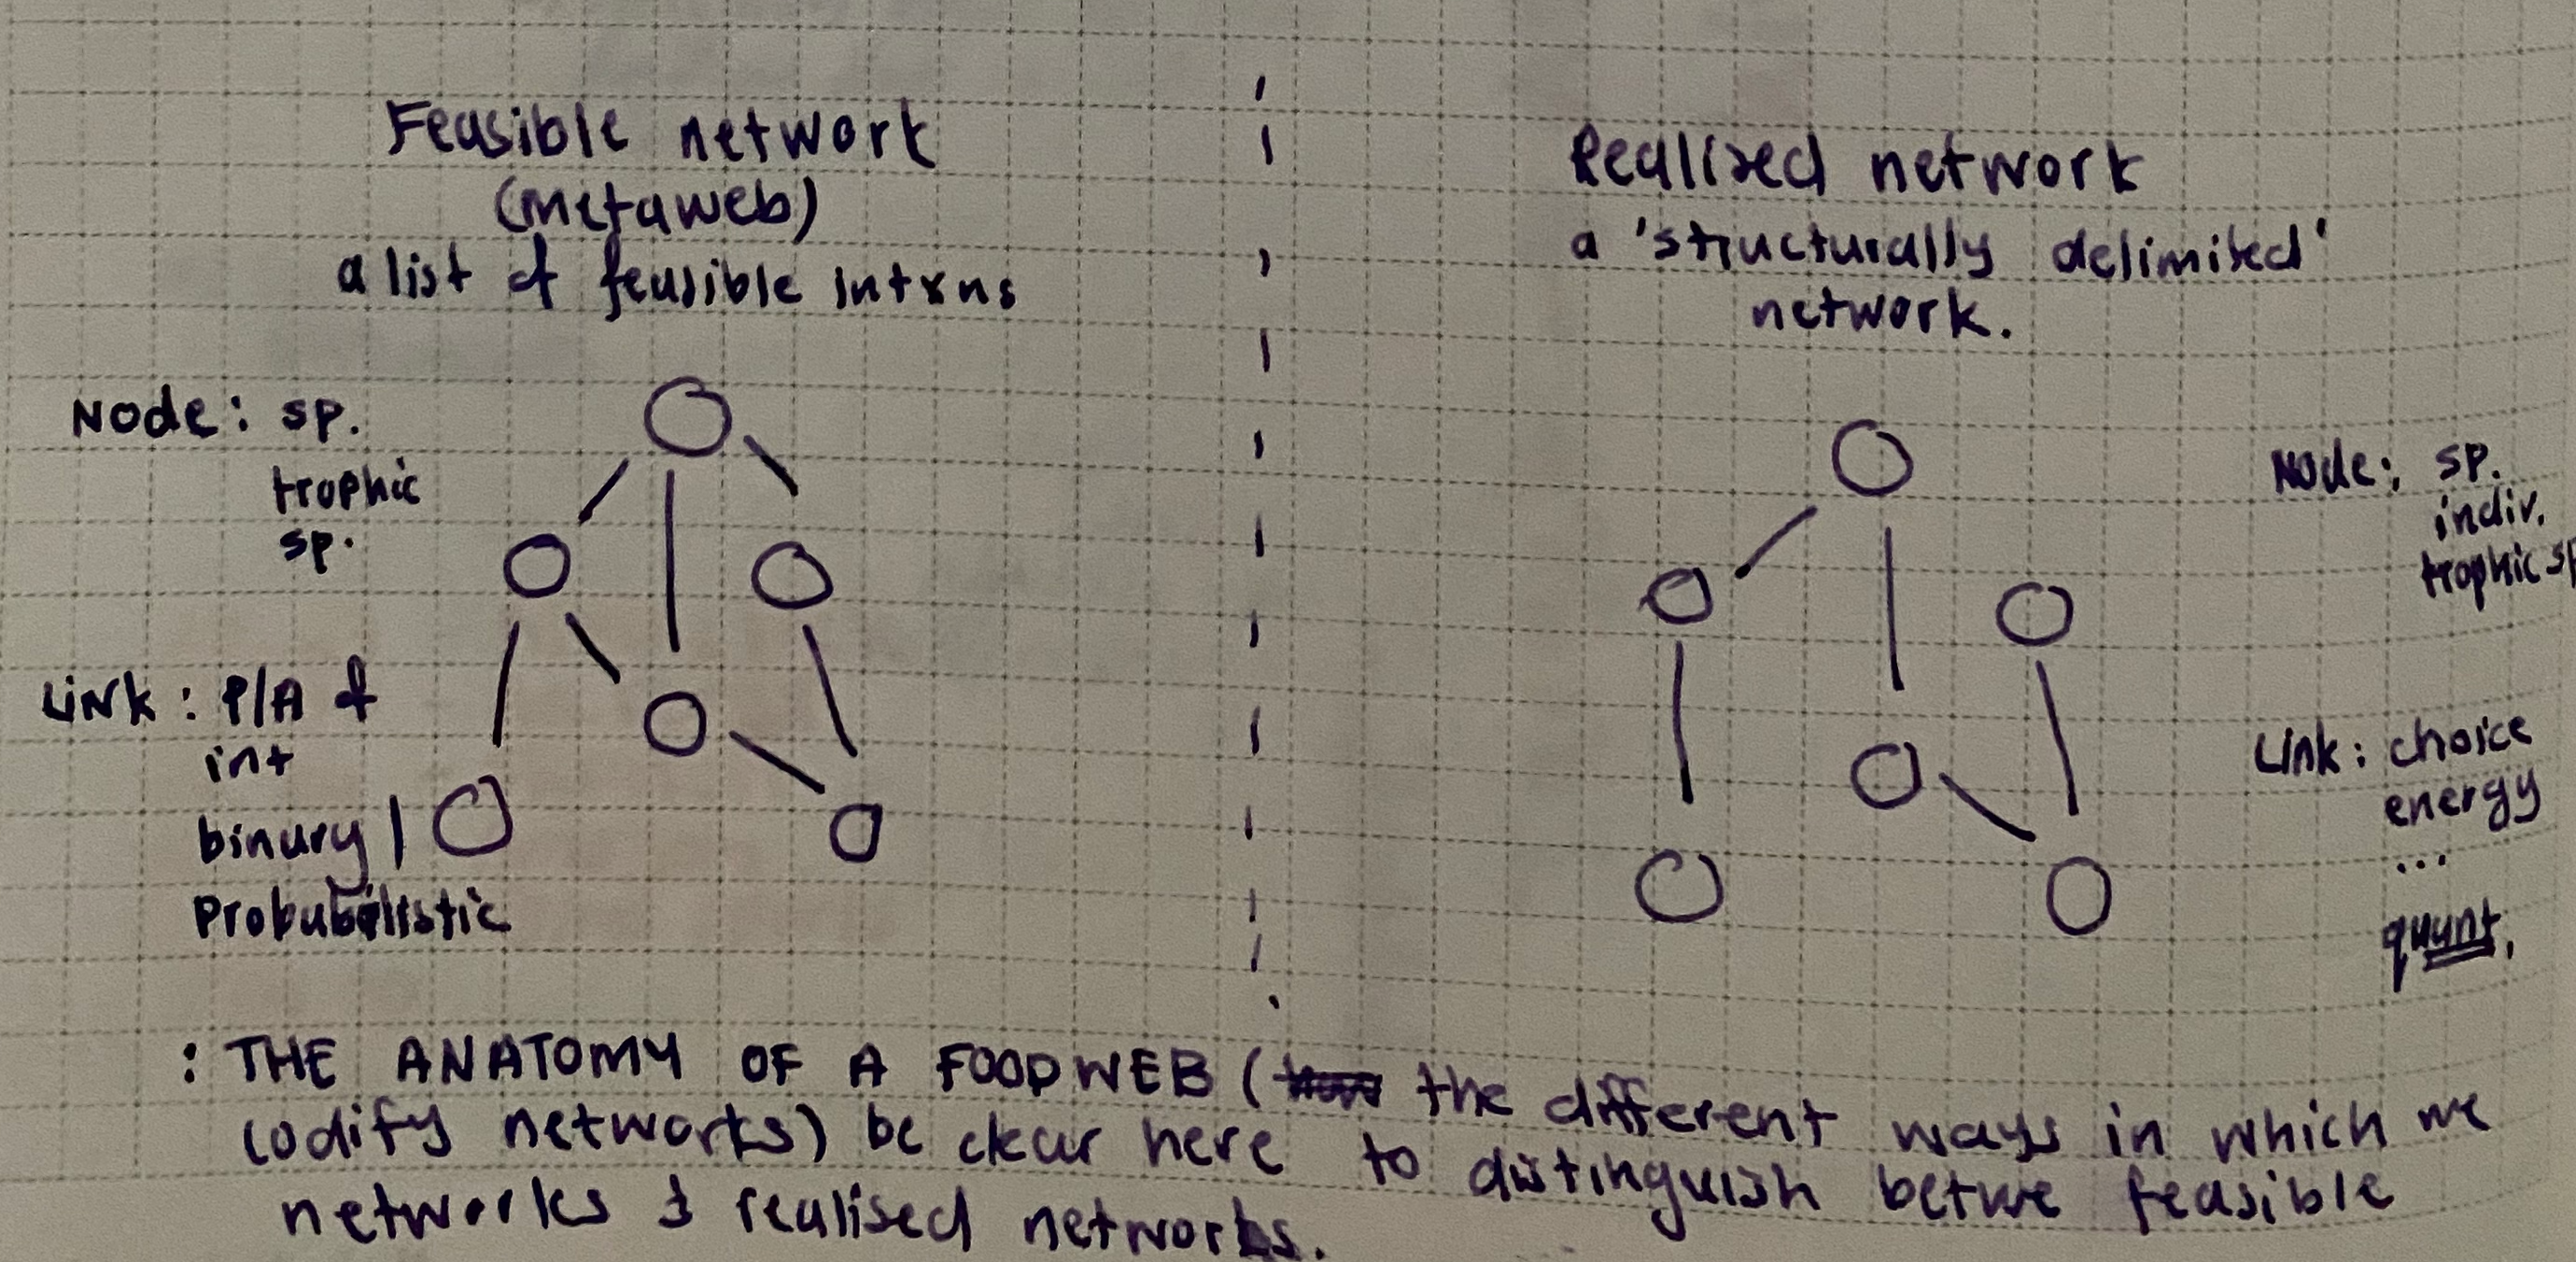
\includegraphics{images/anatomy.png}

}

\caption{\label{fig-anatomy}The many ways in which a food web can be
defined and described at the node, edge, and even network level.}

\end{figure}%

\subsubsection{How do we define a node?}\label{how-do-we-define-a-node}

Although this may seem an elementary question in the context of food
webs --- a node \emph{should} represent a (taxonomic) species, the
reality is that nodes can often represent an aggregation of different
species - so called `trophic species' or segregation of species by life
stages. Representing nodes as non-taxonomic species can be useful in
certain contexts (Williams \& Martinez, 2000; Yodzis, 1982) and in cases
where the adult and larval stages of a species have different diets it
may make ecological sense (Clegg et al., 2018) meaning that it is not
uncommon that networks often have nodes that have different definitions
of a `species' \emph{e.g.} consisting of both taxonomic and trophic
species. Practical implications of how we are aggregating the nodes is
that the resolution may not always be `pixel perfect' \emph{i.e.,} we
may be unable to assess the co-extinction risk of a species pair,
however there is value in having nodes that represent an aggregation of
species, as these convey a much more general overview of how the links
are distributed within the community.

\subsubsection{What is meant by an
edge?}\label{what-is-meant-by-an-edge}

At its core, links within food webs can be thought of as a
representation of either feeding links between species - be that
realised (Pringle, 2020) or potential (Dunne, 2006), or representative
of fluxes within the community/system \emph{e.g.,} energy transfer or
material flow (Lindeman, 1942). How we specify links will influence the
resulting structure of the network - and the inferences we will make
thereof. For example taking a food web that consists of links
representing all \emph{potential} feeding links for a community
(\emph{i.e.,} a metaweb) will be meaningless if one is interested in
understanding the flow of energy through the network as the links within
a metaweb do not represent environmental/energetic constraints. In
addition to the various ways of defining the links between species pairs
there are also a myriad of ways in which the links themselves can be
quantified. Links between species are often treated as being present or
absent (\emph{i.e.,} binary) but it is also possible to use
probabilities (Banville et al., 2024; which quantifies how likely an
interaction is to occur, Poisot, Cirtwill, et al., 2016) or continuous
measurements (which quantifies the strength of of an interaction, Berlow
et al., 2004).

\subsubsection{Putting the parts
together}\label{putting-the-parts-together}

The ingredients one uses to construct networks generates a unique
representation of the mechanisms (see Section~\ref{sec-mechanisms}) that
allow inference and reasoning about the structure, aspects of dynamics
(\emph{e.g.,} stability), and potentially the function of communities
(\emph{e.g.,} flux). It is thus important to keep in mind that different
networks are going to be representing different processes and that can
only be used for inference of some but not all aspects of the community
at large. Here it may be meaningful to contextualise the different
`types' of food webs within the larger research programmes (or even
practical needs) that have been driving the construction of them.

Before thinking about the ways in which we can predict networks it is
perhaps meaningful to take a step back and think about the different
criteria that must be met in order for an interaction to be able to
occur between two species, specifically thinking of this in terms of
distinguishing between the feasibility versus realisation of an
interaction and how these are determined (and defined by) different
`rules'/mechanisms. If we look at this feasibility-reality continuum
(Figure~\ref{fig-feasibility}) it is clear how the different predictive
approaches (methods) tend to fall within one of the broader categories
identified (distinguished) in the triangle. This is not to say that this
shortcoming should be viewed as a `bug' but rather a `feature' of the
field as it allows one to engage with, as well as construct networks at
different scales, which is particularly valuable if one takes into
consideration the considerable `data cost' of predicting well resolved,
realised networks in comparison to constructing high-level metawebs.
However, it is important that there is an awareness and acknowledgement
of where within this feasibility-reality one is working at and how this
will impact and limit the contexts in which the resulting network can be
used and applied within.

\section{From Nodes and Edges to Scales, Context, and
Processes}\label{sec-mechanisms}

Armed with these basics, it is now possible to review the scales and
assumptions that are made by a wide range of tools to assist in
constructing networks against poor data with the hope of capturing
important processes that underpin accurate prediction. Our thesis
centres on a four-tier conceptualization of networks: co-occurrence,
feasibility, mass effects and energetics. In the following sections we
review each of these and then provide a synthesis among them.

\subsection{Understanding the processes that determine species
interactions}\label{sec-process}

Processes that are all-or-nothing (possibility) vs processes that are
context dependent (likelihood). Processes form the underlying logic of
models (and arguably even empirical data capture). Processes influence
how we define the network (its anatomy). Ultimately when we put this all
together it will influence how we can and should use the resulting
network.

Important goal here is to introduce the idea that there are multiple
facets as to what determines the interaction between species and that
there is some sort of `scale of organisation'
Figure~\ref{fig-feasibility}. We can then introduce these different
scales/theories and I think some key points to highlights are the
features, limits, and descriptions of these different scales (by that I
mean what rules them, what finds them, and what binds them - sorry not
sorry). I think it is also worth either in this section or in the one
where we talk about model families to discuss the idea of `moving
between' different levels - e.g.~downsampling but also feasibility - can
we actually do that? Another interesting discussion here (or maybe
actually something that can make its way into the concluding remarks) is
thinking about what determines interactions vs what determines
structure\ldots{}

\begin{itemize}
\tightlist
\item
  These different theories are shown in Figure~\ref{fig-feasibility} and
  we can see there is some element of scaling (species - population -
  individual)
\end{itemize}

\begin{figure}

\centering{

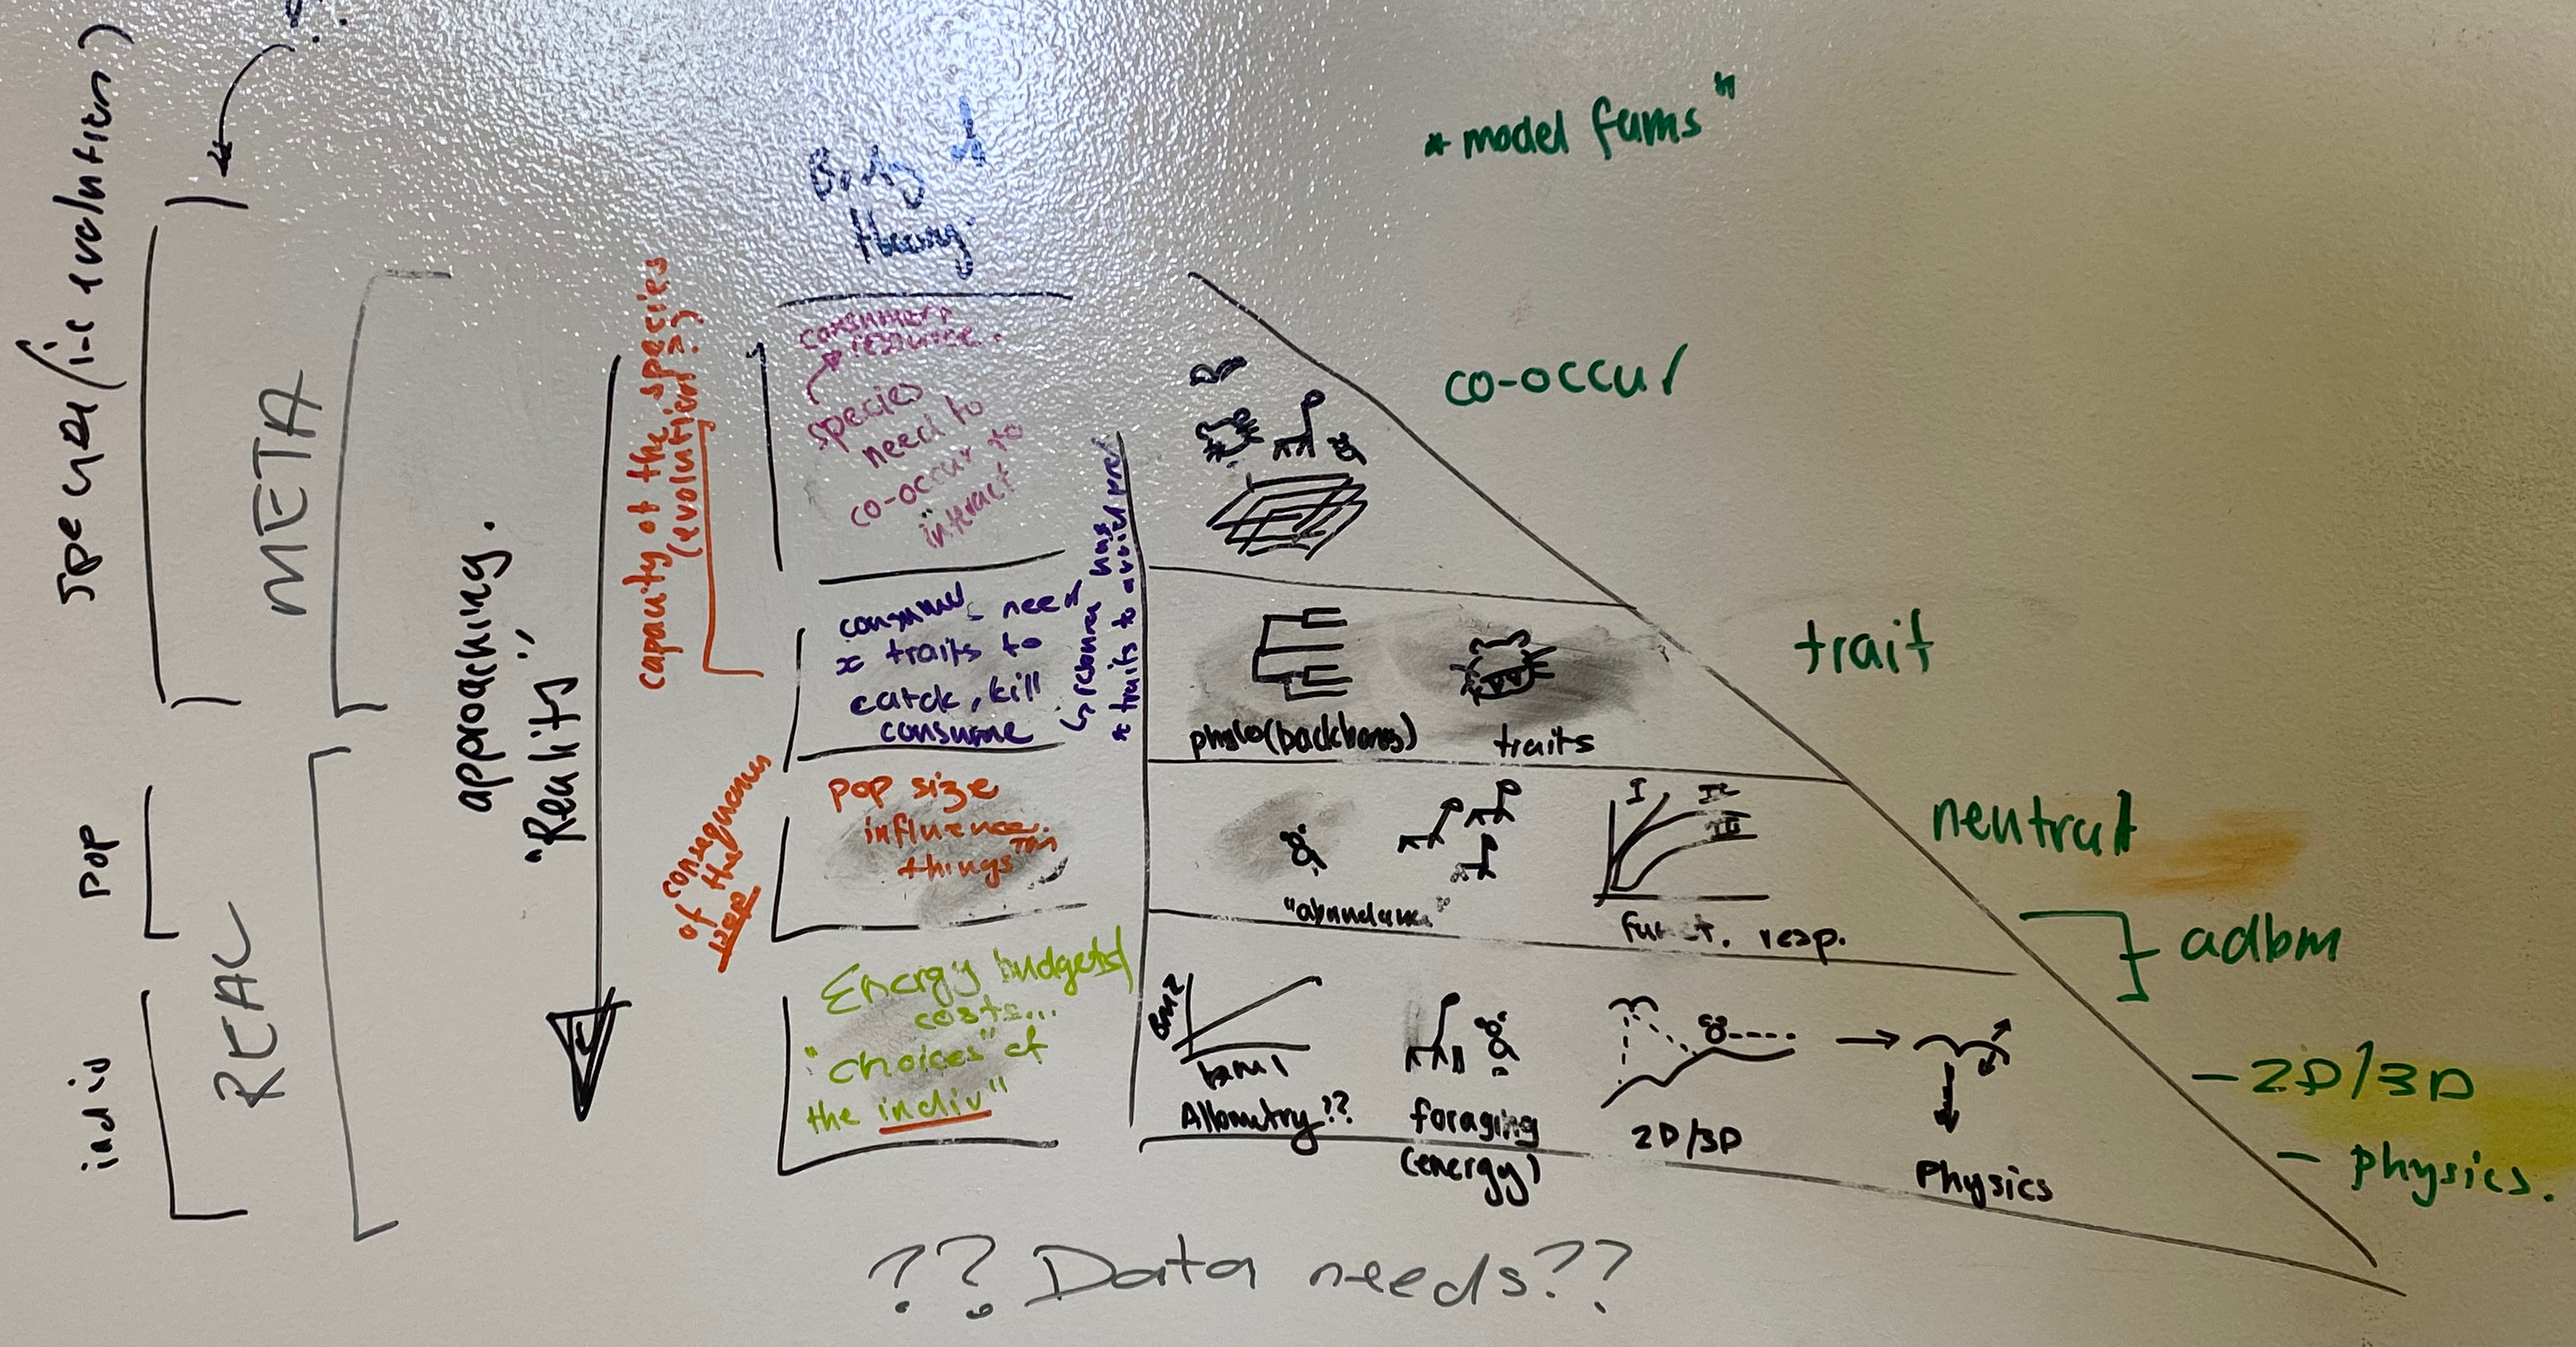
\includegraphics{images/concept_v2.png}

}

\caption{\label{fig-feasibility}TODO.}

\end{figure}%

\textbf{Evolutionary compatibility}

There is compelling evidence that the possibility of an interaction
occurring between two species is the result of their shared
(co)evolutionary history (Dalla Riva \& Stouffer, 2016; Gómez et al.,
2010). In the more proximal sense this is manifested as the `trait
complementarity' between two species, whereby one species (the predator)
has the `correct' set of traits that allow it to chase, capture, kill,
and consume the other species (the prey). For species pairs where this
condition is not met the link is deemed to be forbidden (Jordano,
2016b); \emph{i.e.,} not physically possible and will always be absent
within the network. In the context of trying to determine the
feasibility (\emph{i.e.,} the \emph{possibility}) of an interaction,
phylogeny is an excellent predictor (Fricke et al., 2022; Strydom et
al., 2022) and allows one to construct what can be considered to be a
metaweb. In terms of thinking about the anatomy of an `feasibility
network' one should be aware that it is possible to represent
interactions as either binary (feasible/forbidden; \emph{i.e.,} the
traditional definition of a metaweb Dunne (2006)) or as a probability
(Banville et al., 2024), where the probability represents how likely
that the interaction between to species is feasible (what is the
possibility of this interaction occurring?).

\textbf{(Co)occurrence}

Although the outright assumption that because two species are
co-occurring it must mean that they are interacting is inherently flawed
(Blanchet et al., 2020), it is of course impossible for two species to
interact (at least in terms of feeding links) if they are not
co-occurring in time and space. Thus co-occurrence data alone is
insufficient to build an accurate and ecologically meaningful
representation of a food web having information on the co-occurrence of
species can further aid us in refining metawebs by allowing us to
downsample the network based on the species found in a specific
location, or even add additional uncertainty based in how likely species
are to co-occur (Dansereau et al., 2023). Additionally the interplay
between the interaction between a species pair and their co-occurrence
is meaningful when one is operating in the space of trying to determine
the distribution of a species (Higino et al., 2023), and forms a key
component of some of the next generation species distribution models
\emph{e.g.,} joint SDMs (Pollock et al., 2014).

\textbf{Abundance}

The abundance of the different species within the community can
influence the likelihood of an interaction occurring in a myriad of
ways. There is the argument that networks (and the interactions that
make them up) are driven by only the abundance of the different species
and not the characteristics (traits), \emph{sensu} neutral processes and
have been formalised with the neutral model (Canard et al., 2012), as
well as statistical tools (Momal et al., 2020). Alternatively the
abundance of species in a community can influence which interactions are
ultimately realised (Banville et al., 2024; Poisot et al., 2015).

\textbf{Predator choice (energetic cost)}

Ultimately, predator choice is underpinned by the energetic cost-benefit
of trying to catch, kill, and consume prey, and is well described within
optimal foraging theory {[}ref{]} and rests on the idea that the prey a
predator chooses to target is one that will have the greatest return on
energy with the lowest energetic cost. There are additional bodies of
work that attempt to include the cost of movement that the environment
imposes on an individual (Cherif et al., 2024) as well as 2D/3D search
space (Pawar et al., 2012). In terms of formalising these processes in
the context of predicting networks using diet models (Beckerman et al.,
2006; Petchey et al., 2008) that have predator choice determined by the
handling time, energy content, prey density, and predator attack rate.
Wootton et al. (2023) developed a model that moves the energy of the
system into different modules related to the process of the predator
acquiring energy from the prey \emph{i.e.,} compartmentation in food
webs (Krause et al., 2003).

\textbf{Indirect interactions}

The realisation (presence/absence) or strength of trophic interactions
themselves can also be modified by other, indirect (non-trophic),
interactions (Golubski \& Abrams, 2011; Pilosof et al., 2017), this can
be either `directly' through \emph{e.g.,} competition or `indirectly'
\emph{e.g.,} mutualistic/facilitative interactions will alter the
fine-scale distribution and abundance of some species (Kéfi et al.,
2012, 2015).

It should be self evident that the different processes discussed above
are all ultimately going to influence the realisation of interactions as
well as the structure of a network, however they are acting at different
scales of organisation. Both the \textbf{co-occurrence} and the
\textbf{evolutionary compatibility} are valid at the scale of the
species pair of interest, that is the \emph{possibility} of an
interaction being present/absent is assessed at the pairwise level and
one is left with a `list' of interactions that are present/absent.
Although it is possible to build a network (\emph{i.e.,} metaweb) from
this information it is important to be aware that the structure of this
network is not constrained by real-world dynamics or conditions, just
becuase species are able to interact does not mean that they will
(Poisot et al., 2015). In order to construct a network who's structure
is a closer approximation of reality (localised interactions) one needs
to take into consideration properties of the community as a whole and
not just the two species of interest.

\textbf{downsampling paragraph??}

\section{Network prediction is
nuanced}\label{network-prediction-is-nuanced}

The different models that are used to either predict or construct
networks have an underlying philosophy that often only captures one or a
few of the processes discussed in Section~\ref{sec-process}, has
implications for how the resulting network is defined
Section~\ref{sec-anatomy}, which will ultimately delimit and define what
inferences can be made from the resulting network. Selecting a model for
the task of network prediction should come down to two things; what
\emph{aspect} of a food web one is interested in predicting, and what
data are available, necessary, and sufficient, and what is the purpose
of wanting to predict a network? It is important that a researcher is
aware of this to ensure that the appropriate model is selected. Broadly
researchers will be interested in predicting/constructing two different
types of networks; \emph{metawebs}, which is essentially a list of all
interactions that are \emph{possible} for a specific community
(\emph{i.e.,} at the scale of the species pairs), or being able to
predict location specific, \emph{realised}, networks for the community
(\emph{i.e.,} at the scale of the community). The nature of metawebs
means that they are unable to capture the structural metrics of
realised/`real-world' networks (Caron et al., 2024). The researcher is
also constrained by the data needs of both the model as well as the
network type; for example in order to predict a realised network one
needs additional data (\emph{e.g.,} abundance), making metawebs a more
feasible choice in data-poor contexts (\emph{e.g.,} Strydom et al.
(2023) construct a metaweb using a species list and a phylogenetic
tree). The final question is assessing the purpose of predicting a
network - is it to create a series of simulated, species agnostic but
still ecologically plausible, networks {[}\emph{e.g.,}{]} or to predict
a network for a specific community at a specific location. It is these
three points that will ultimately dictate which model is going to best
allow one to predict the appropriate network.

\begin{quote}
Although the ability to predict `real-world' interactions (and the
resulting food webs) can have more intuitive `real world' applications
\emph{e.g.,} being able to `recover' food webs that have since gone
extinct (Dunne et al., 2008; Yeakel et al., 2014), using pairwise
interactions to understand species distributions (Pollock et al., 2014)
or even co-extinction risk (Dunn et al., 2009), a more structural
approach to network construction affords one an opportunity to
interrogate some of the more high-level mechanisms that are structuring
networks.
\end{quote}

\subsection{Models that predict structure}\label{sec-network-build}

Although we identify mechanisms that determine species interactions in
Section~\ref{sec-process} not all models that are used to predict
networks operate at this `mechanistic' level, but rather represent the
\emph{structure} of a network based on a series of \emph{a priori}
assumptions of network connectance (\emph{e.g.,} the niche model
Williams \& Martinez (2000); although see Allesina \& Pascual (2009) for
a parameter-free model) or other structural features of a
\emph{realised} network (\emph{e.g.,} stochastic block model, Xie et al.
(2017)). Importantly these structural models do not make species
specific predictions (they are species agnostic and usually treat nodes
as trophic species) and so cannot be used to determine if an interaction
is either possible \emph{or} realised between two species
(\emph{i.e.,}one cannot use these models to determine if species \(a\)
eats species \(b\)). Although this means this suite of models are
unsuitable as tools for predicting interactions, they have been shown to
be sufficient tools to predict the structure of networks (Williams \&
Martinez, 2008).

\subsection{How do we predict food
webs?}\label{how-do-we-predict-food-webs}

There as many ways to predict networks as what there is to define them
and along with taking into consideration the points raised in the
previous section it is also beneficial to think about the context in
which the different models were developed - and how this will influence
the networks that they produce\ldots{} Also it is not feasibly possible
to list every single approach that has been developed to predict
networks and so we will present what we believe to be the broad families
that represent the different approaches to predicting networks,
particularly how these relate to the processes identified in
Section~\ref{sec-process}, as well as models that predict network
structure (see Section~\ref{sec-network-build}).

In order for a model to formalise a `complete' food web it is necessary
to formalise two aspects of the network, `who eats whom' (to determine
the links between nodes) as well as the structure of the network (to
limit the distribution of links), however most models are inclined to
focus on one of the two aspects. As there are many food web models to
choose from it is perhaps useful to think about the models in terms of
model families, a summary of these families is presented in
Table~\ref{tbl-families} highlights the differences and similarities of
the philosophies and assumptions that determine a network. A more
extensive overview of the different models that fall with in the
different model families can be found in
\href{https://beckslab.github.io/ms_t_is_for_topology/notebooks/model_descriptions-preview.html}{SuppMat
1} and for a more detailed breakdown of the different `traits' of the
model families refer to
\href{https://beckslab.github.io/ms_t_is_for_topology/notebooks/model_qualitative-preview.html}{SuppMat
2}.

\begin{longtable}[]{@{}
  >{\raggedright\arraybackslash}p{(\columnwidth - 10\tabcolsep) * \real{0.1622}}
  >{\raggedright\arraybackslash}p{(\columnwidth - 10\tabcolsep) * \real{0.1892}}
  >{\raggedright\arraybackslash}p{(\columnwidth - 10\tabcolsep) * \real{0.1622}}
  >{\raggedright\arraybackslash}p{(\columnwidth - 10\tabcolsep) * \real{0.1622}}
  >{\raggedright\arraybackslash}p{(\columnwidth - 10\tabcolsep) * \real{0.1622}}
  >{\raggedright\arraybackslash}p{(\columnwidth - 10\tabcolsep) * \real{0.1622}}@{}}
\caption{A summary of the different families of tools that can be used
to generate food webs.}\label{tbl-families}\tabularnewline
\toprule\noalign{}
\begin{minipage}[b]{\linewidth}\raggedright
Model family
\end{minipage} & \begin{minipage}[b]{\linewidth}\raggedright
Assumptions
\end{minipage} & \begin{minipage}[b]{\linewidth}\raggedright
Data/process
\end{minipage} & \begin{minipage}[b]{\linewidth}\raggedright
`Limitation'
\end{minipage} & \begin{minipage}[b]{\linewidth}\raggedright
Network type
\end{minipage} & \begin{minipage}[b]{\linewidth}\raggedright
Key reference
\end{minipage} \\
\midrule\noalign{}
\endfirsthead
\toprule\noalign{}
\begin{minipage}[b]{\linewidth}\raggedright
Model family
\end{minipage} & \begin{minipage}[b]{\linewidth}\raggedright
Assumptions
\end{minipage} & \begin{minipage}[b]{\linewidth}\raggedright
Data/process
\end{minipage} & \begin{minipage}[b]{\linewidth}\raggedright
`Limitation'
\end{minipage} & \begin{minipage}[b]{\linewidth}\raggedright
Network type
\end{minipage} & \begin{minipage}[b]{\linewidth}\raggedright
Key reference
\end{minipage} \\
\midrule\noalign{}
\endhead
\bottomrule\noalign{}
\endlastfoot
null & Links are randomly distributed within a network & & parameter
assumptions, species agnostic & structural network & \\
neutral & Network structure is random, but species abundance determines
links between nodes & abundance & parameter assumptions & structural
network & Canard et al. (2012) \\
resource & Networks are interval, species can be ordered on a `niche
axis' & & parameter assumptions, species agnostic & structural network &
Williams \& Martinez (2008) \\
generative & Networks are determined by their structural features & &
need real world networks & structural network & \\
energetic & Interactions are determined by energetic costs & abundance +
energy & does not account for forbidden links in terms of evolutionary
compatibility & `energy' network & \\
graph embedding & Interactions can be predicted from the latent traits
of networks & evolutionary compatibility & need real world networks &
metaweb & Strydom et al. (2023) \\
trait matching & Interactions can be inferred by a mechanistic
framework/relationships & evolutionary compatibility & well studied
species/communities & metaweb & Morales-Castilla et al. (2015) \\
binary classifiers & Interactions can be predicted by learning the
relationship between interactions and ecologically relevant predictors &
evolutionary compatibility & need real world networks & metaweb &
Pichler et al. (2020) \\
expert knowledge & `Boots on the ground' ecological knowledge and
observations & evolutionary compatibility & well studied
species/communities & metaweb & \\
data scavenging & Webscraping to create networks from online databases &
& need real world networks & metaweb & Poisot, Gravel, et al. (2016) (if
you squint?) \\
co-occurrence & co-occurrence patterns arise from interactions so we can
use these patterns to reverse engineer the interactions & co-occurrence
& does not account for forbidden links in terms of evolutionary
compatibility or account for energy constraints & co-occurrence network
& \\
\end{longtable}

\section{Making Progress with
Networks}\label{making-progress-with-networks}

There is a bit of a `point of conflict' between those calling for `pixel
perfect', regional scale data (Pringle, 2020; Pringle \& Hutchinson,
2020) and for the means to generate networks that are ecologically
plausible \emph{representations} (\emph{sensu} structural networks).
This represents two challenges; one is that models that represent
generalisations often lack the ability to retrieve any species/community
specificity which limits their utility for real world, species-driven
scenarios \emph{e.g.,} species driven conservation efforts, however
networks that are constructed through either empirical observations or
through predictive means are fundamentally going to represent metawebs,
\emph{i.e.,} lack constrained links.

In this section I want to highlight that we don't actually have any
clear guidelines as to how we can `use' networks - which probably stems
from both the fact that when I am talking about a network and when
someone else is talking about a network we may actually be talking about
two very different conceptualisations of `a network' (this should
actually be a selling point in the intro - may have just found my
\emph{raison d'etre}) as well as that a lot of the ideas that we have
about networks are not really tied to any sort of tangible function
(i.e.~Tim's GeoBon ms thing-y). However we can maybe at least try to
present some guidelines - but I think specifically within the sort of
Petchey dilemma space and clearly tied to the ideas we discuss in the
ms. This includes: understanding the limits of how a network is defined
and how the underlying theory impacts the use as well as data?? IDK we
need to shoehorn data in here somehow\ldots{} We can also use this as a
gap identifying space and I think the framing can still rest under the
limits concept particularly time, space, and boundaries - which will all
probably fall under some aspect of biological scale\ldots{} We can also
raise the idea of trust - as in which methods have more support/trust
than others. Also what even a `real' network entails (and this links
again back to Tim's stuff) as well as a subtle jab at Pringles notion
that the most critical issue in the world of food webs is being able to
identify every. single. link. even though there is no real discussion as
to what is an `opportunistic' link vs a link that represents a
sustainable energy source for a population (or would it be an
individual)\ldots{}

We need to be aware of the parameter space that is possible given a
specific definition of a network and operate within those parameters.

\section{Concluding remarks}\label{concluding-remarks}

I think the idea of time and how we are aggregating networks across that
should be a prominent feature here\ldots{}

\begin{itemize}
\item
  In certain situations structure is `enough' but there may be use cases
  where we are really interested in the node-level interactions
  \emph{i.e.,} species identity is a thing we care about and need to be
  able to retrieve specific interactions at specific nodes correctly.
\item
  Why do interaction models do so badly at predicting structure? Nuance
  of metaweb vs realisation but also time? At the core of it interaction
  models are trained on existing interaction data; this is data that are
  most likely closer to a metaweb than a local realisation even if they
  are being inventoried at a small scale\ldots{}

  \begin{itemize}
  \tightlist
  \item
    We can briefly shoehorn downsampling here maybe??
  \end{itemize}
\item
  It will be interesting to bring up the idea that if a model is missing
  a specific pairwise link but doing well overall then when does it
  matter?

  \begin{itemize}
  \item
    The fact that \emph{some} people are concerned about the taxonomic
    resolution and cascading effects those might have on our
    understanding of network structure (Pringle, 2020; Pringle \&
    Hutchinson, 2020), but that puts us in a place where we are at risk
    of losing our ability to distinguish the wood from the tree - are we
    not (at least at times) concerned more with understanding ecosystem
    level processes than with needing to understand things
    \emph{perfectly} at the species level.
  \item
    I don't think these `rare'/nuanced links (e.g.~carnivorous hippos)
    are going to rock the boat when we think about networks at the
    structural level.
  \end{itemize}
\end{itemize}

\begin{quote}
``The resolution of food-web data is demonic because it can radically
change network topology and associated biological inferences in ways
that are unknowable in the absence of better data.'' - Pringle \&
Hutchinson (2020) The counter to this is that structural models are
often not working at the species level and thus the structure remains
`unchanged' when you increase the resolution - I don't think that people
are that concerned with the structure of real world networks barring
connectance and since that scales with species richness anyway your
final proportion will probably still remain the same\ldots{}
\end{quote}

\begin{itemize}
\item
  I think a big take home will (hopefully) be how different approaches
  do better in different situations and so you as an end user need to
  take this into consideration and pick accordingly. I think Petchey et
  al. (2011) might have (and share) some thoughts on this. I feel like I
  need to look at Berlow et al. (2008) but maybe not exactly in this
  context but vaguely adjacent.

  \begin{itemize}
  \tightlist
  \item
    I think this is sort of the crux of the argument presented in
    Brimacombe et al. (2024) as well.
  \end{itemize}
\end{itemize}

\begin{quote}
\emph{``we highlight an interesting paradox: the models with the best
performance measures are not necessarily the models with the closest
reconstructed network structure.''} - Poisot (2023)
\end{quote}

\begin{itemize}
\item
  Do we need network models to predict interactions and interaction
  models to predict structure?

  \begin{itemize}
  \item
    ``Another argument for the joint prediction of networks and
    interactions is to reduce circularity and biases in the predictions.
    As an example, models like linear filtering generate probabilities
    of non-observed interactions existing, but do so based on measured
    network properties.'' - Strydom et al. (2021)
  \item
    Aligning (dove-tailing) with this the idea of ensemble modelling as
    presented by Becker et al. (2022)
  \end{itemize}
\item
  Close out with a call to action that we have models that predict
  networks very well and models that predict interactions very well but
  nothing that is doing well at predicting both - this is where we
  should be focusing our attention when it comes to furthering model
  development\ldots{}
\item
  Do we expect there to be differences when thinking about unipartite vs
  bipartite networks? Is there underlying ecology/theory that would
  assume that different mechanisms (and thus models) are relevant in
  these two `systems'.

  \begin{itemize}
  \tightlist
  \item
    The Terry \& Lewis (2020) paper looks at some methods but is
    specifically looking at a bipartite world\ldots{}
  \end{itemize}
\end{itemize}

do we bring this up? this could be a box\ldots{} if we have the
`finances' for it\ldots{} otherwise it should go to the outstanding
questions fur sure

``That being said, there is a compelling argument for the need to
`combine' these smaller functional units with larger spatial networks
(Fortin et al., 2021) and that we should also start thinking about the
interplay of time and space (Estay et al., 2023). Although deciding
exactly what measure might actually be driving differences between local
networks and the regional metaweb might not be that simple (Saravia et
al., 2022).''

\subsection{Time}\label{time}

Look at Hutchinson et al. (2019) and in a way Rooney et al. (2008)

We lack a clear agenda (and conceptualisation) as to what the
appropriate level of aggregation is for a `network'. Realistically most
empirical networks are more aligned with `feasibility networks' as
opposed to `realised networks' as they are often the result of some sort
of aggregation of observations across time. This `problem' is two-fold.
Firstly we need to think about how this affects any sort of development
of theory that sits closer to the `realised network' side of the
spectrum - how often are we trying to ask and answer questions about
realised networks using feasible networks? The second is that this lack
of `direction' as to how we should define a network is (actually)
probably one of the biggest barriers that is affecting the use of
networks in applied settings\ldots{}

Another time perspective question is when do we determine a link to be
`real'\ldots{} In the context of feasible networks this is perhaps
clearer - all things equal would the predator be bale to consume the
prey. However in the realised space there is also the question of the
long term `energetic feasibility' of an interaction - just because an
interaction is possible in the now is it able to sustain a population in
the long term. And what is the scale for that long term - are we
thinking at the generational scale? Because ultimately when we are
constructing a network we are aggregating not only across space but also
across time.

\section*{Outstanding questions}\label{outstanding-questions}
\addcontentsline{toc}{section}{Outstanding questions}

\begin{itemize}
\item
  non-consumptive effects
\item
  how do we define the spatial and temporal `boundaries' of a network?
\item
  how do we define a `real' network?
\end{itemize}

\section*{References}\label{references}
\addcontentsline{toc}{section}{References}

\phantomsection\label{refs}
\begin{CSLReferences}{1}{0}
\bibitem[\citeproctext]{ref-allesinaFoodWebModels2009}
Allesina, S., \& Pascual, M. (2009). Food web models: A plea for groups.
\emph{Ecology Letters}, \emph{12}(7), 652--662.
\url{https://doi.org/10.1111/j.1461-0248.2009.01321.x}

\bibitem[\citeproctext]{ref-banvilleDecipheringProbabilisticSpecies2024}
Banville, F., Strydom, T., Blyth, P., Brimacombe, C., Catchen, M. D.,
Dansereau, G., Higino, G., Malpas, T., Mayall, H., Norman, K., Gravel,
D., \& Poisot, T. (2024). \emph{Deciphering probabilistic species
interaction networks}. EcoEvoRxiv. \url{https://doi.org/10.32942/X28G8Z}

\bibitem[\citeproctext]{ref-beckerOptimisingPredictiveModels2022}
Becker, D. J., Albery, G. F., Sjodin, A. R., Poisot, T., Bergner, L. M.,
Chen, B., Cohen, L. E., Dallas, T. A., Eskew, E. A., Fagre, A. C.,
Farrell, M. J., Guth, S., Han, B. A., Simmons, N. B., Stock, M.,
Teeling, E. C., \& Carlson, C. J. (2022). Optimising predictive models
to prioritise viral discovery in zoonotic reservoirs. \emph{The Lancet
Microbe}, \emph{3}(8), e625--e637.
\url{https://doi.org/10.1016/S2666-5247(21)00245-7}

\bibitem[\citeproctext]{ref-beckermanForagingBiologyPredicts2006}
Beckerman, A. P., Petchey, O. L., \& Warren, P. H. (2006). Foraging
biology predicts food web complexity. \emph{Proceedings of the National
Academy of Sciences}, \emph{103}(37), 13745--13749.
\url{https://doi.org/10.1073/pnas.0603039103}

\bibitem[\citeproctext]{ref-berlowGoldilocksFactorFood2008}
Berlow, E. L., Brose, U., \& Martinez, N. D. (2008). The {``{Goldilocks}
factor''} in food webs. \emph{Proceedings of the National Academy of
Sciences}, \emph{105}(11), 4079--4080.
\url{https://doi.org/10.1073/pnas.0800967105}

\bibitem[\citeproctext]{ref-berlowInteractionStrengthsFood2004}
Berlow, E. L., Neutel, A.-M., Cohen, J. E., de Ruiter, P. C., Ebenman,
B., Emmerson, M., Fox, J. W., Jansen, V. A. A., Iwan Jones, J.,
Kokkoris, G. D., Logofet, D. O., McKane, A. J., Montoya, J. M., \&
Petchey, O. (2004). Interaction strengths in food webs: Issues and
opportunities. \emph{Journal of Animal Ecology}, \emph{73}(3), 585--598.
\url{https://doi.org/10.1111/j.0021-8790.2004.00833.x}

\bibitem[\citeproctext]{ref-blanchetCooccurrenceNotEvidence2020}
Blanchet, F. G., Cazelles, K., \& Gravel, D. (2020). Co-occurrence is
not evidence of ecological interactions. \emph{Ecology Letters},
\emph{23}(7), 1050--1063. \url{https://doi.org/10.1111/ele.13525}

\bibitem[\citeproctext]{ref-brimacombeApplyingMethodIts2024}
Brimacombe, C., Bodner, K., \& Fortin, M.-J. (2024). \emph{Applying a
method before its proof-of-concept: {A} cautionary tale using inferred
food webs}. \url{https://doi.org/10.13140/RG.2.2.22076.65927}

\bibitem[\citeproctext]{ref-brimacombeShortcomingsReusingSpecies2023}
Brimacombe, C., Bodner, K., Michalska-Smith, M., Poisot, T., \& Fortin,
M.-J. (2023). Shortcomings of reusing species interaction networks
created by different sets of researchers. \emph{PLOS Biology},
\emph{21}(4), e3002068.
\url{https://doi.org/10.1371/journal.pbio.3002068}

\bibitem[\citeproctext]{ref-canardEmergenceStructuralPatterns2012}
Canard, E., Mouquet, N., Marescot, L., Gaston, K. J., Gravel, D., \&
Mouillot, D. (2012). Emergence of {Structural Patterns} in {Neutral
Trophic Networks}. \emph{PLOS ONE}, \emph{7}(8), e38295.
\url{https://doi.org/10.1371/journal.pone.0038295}

\bibitem[\citeproctext]{ref-caronTraitmatchingModelsPredict2024}
Caron, D., Brose, U., Lurgi, M., Blanchet, F. G., Gravel, D., \&
Pollock, L. J. (2024). Trait-matching models predict pairwise
interactions across regions, not food web properties. \emph{Global
Ecology and Biogeography}, \emph{33}(4), e13807.
\url{https://doi.org/10.1111/geb.13807}

\bibitem[\citeproctext]{ref-cherifEnvironmentRescueCan2024}
Cherif, M., Brose, U., Hirt, M. R., Ryser, R., Silve, V., Albert, G.,
Arnott, R., Berti, E., Cirtwill, A., Dyer, A., Gauzens, B., Gupta, A.,
Ho, H.-C., Portalier, S. M. J., Wain, D., \& Wootton, K. (2024). The
environment to the rescue: Can physics help predict predator--prey
interactions? \emph{Biological Reviews}, \emph{n/a}(n/a).
\url{https://doi.org/10.1111/brv.13105}

\bibitem[\citeproctext]{ref-cleggImpactIntraspecificVariation2018}
Clegg, T., Ali, M., \& Beckerman, A. P. (2018). The impact of
intraspecific variation on food web structure. \emph{Ecology},
\emph{99}(12), 2712--2720. \url{https://doi.org/10.1002/ecy.2523}

\bibitem[\citeproctext]{ref-dallarivaExploringEvolutionarySignature2016}
Dalla Riva, G. V., \& Stouffer, D. B. (2016). Exploring the evolutionary
signature of food webs' backbones using functional traits. \emph{Oikos},
\emph{125}(4), 446--456. \url{https://doi.org/10.1111/oik.02305}

\bibitem[\citeproctext]{ref-dansereauSpatiallyExplicitPredictions2023}
Dansereau, G., Barros, C., \& Poisot, T. (2023). \emph{Spatially
explicit predictions of food web structure from regional level data}.

\bibitem[\citeproctext]{ref-dunnSixthMassCoextinction2009}
Dunn, R. R., Harris, N. C., Colwell, R. K., Koh, L. P., \& Sodhi, N. S.
(2009). The sixth mass coextinction: Are most endangered species
parasites and mutualists? \emph{Proceedings. Biological Sciences},
\emph{276}(1670), 3037--3045.
\url{https://doi.org/10.1098/rspb.2009.0413}

\bibitem[\citeproctext]{ref-dunneNetworkStructureFood2006}
Dunne, J. A. (2006). The {Network Structure} of {Food Webs}. In J. A.
Dunne \& M. Pascual (Eds.), \emph{Ecological networks: {Linking}
structure and dynamics} (pp. 27--86). Oxford University Press.

\bibitem[\citeproctext]{ref-dunneCompilationNetworkAnalyses2008}
Dunne, J. A., Williams, R. J., Martinez, N. D., Wood, R. A., \& Erwin,
D. H. (2008). Compilation and {Network Analyses} of {Cambrian Food
Webs}. \emph{PLOS Biology}, \emph{6}(4), e102.
\url{https://doi.org/10.1371/journal.pbio.0060102}

\bibitem[\citeproctext]{ref-estayEditorialPatternsProcesses2023}
Estay, S. A., Fortin, M.-J., \& López, D. N. (2023). Editorial:
{Patterns} and processes in ecological networks over space.
\emph{Frontiers in Ecology and Evolution}, \emph{11}.

\bibitem[\citeproctext]{ref-fortinNetworkEcologyDynamic2021}
Fortin, M.-J., Dale, M. R. T., \& Brimacombe, C. (2021). Network ecology
in dynamic landscapes. \emph{Proceedings of the Royal Society B:
Biological Sciences}, \emph{288}(1949), rspb.2020.1889, 20201889.
\url{https://doi.org/10.1098/rspb.2020.1889}

\bibitem[\citeproctext]{ref-frickeCollapseTerrestrialMammal2022}
Fricke, E. C., Hsieh, C., Middleton, O., Gorczynski, D., Cappello, C.
D., Sanisidro, O., Rowan, J., Svenning, J.-C., \& Beaudrot, L. (2022).
Collapse of terrestrial mammal food webs since the {Late Pleistocene}.
\emph{Science}, \emph{377}(6609), 1008--1011.
\url{https://doi.org/10.1126/science.abn4012}

\bibitem[\citeproctext]{ref-golubskiModifyingModifiersWhat2011}
Golubski, A. J., \& Abrams, P. A. (2011). Modifying modifiers: What
happens when interspecific interactions interact? \emph{Journal of
Animal Ecology}, \emph{80}(5), 1097--1108.
\url{https://doi.org/10.1111/j.1365-2656.2011.01852.x}

\bibitem[\citeproctext]{ref-gomezEcologicalInteractionsAre2010}
Gómez, J. M., Verdú, M., \& Perfectti, F. (2010). Ecological
interactions are evolutionarily conserved across the entire tree of
life. \emph{Nature}, \emph{465}(7300), 918--921.
\url{https://doi.org/10.1038/nature09113}

\bibitem[\citeproctext]{ref-higinoMismatchIUCNRange2023}
Higino, G. T., Banville, F., Dansereau, G., Muñoz, N. R. F., Windsor,
F., \& Poisot, T. (2023). Mismatch between {IUCN} range maps and species
interactions data illustrated using the {Serengeti} food web.
\emph{PeerJ}, \emph{11}, e14620.
\url{https://doi.org/10.7717/peerj.14620}

\bibitem[\citeproctext]{ref-hutchinsonSeeingForestTrees2019}
Hutchinson, M. C., Bramon Mora, B., Pilosof, S., Barner, A. K., Kéfi,
S., Thébault, E., Jordano, P., \& Stouffer, D. B. (2019). Seeing the
forest for the trees: {Putting} multilayer networks to work for
community ecology. \emph{Functional Ecology}, \emph{33}(2), 206--217.
\url{https://doi.org/10.1111/1365-2435.13237}

\bibitem[\citeproctext]{ref-jordanoChasingEcologicalInteractions2016}
Jordano, P. (2016a). Chasing {Ecological Interactions}. \emph{PLOS
Biology}, \emph{14}(9), e1002559.
\url{https://doi.org/10.1371/journal.pbio.1002559}

\bibitem[\citeproctext]{ref-jordanoSamplingNetworksEcological2016}
Jordano, P. (2016b). Sampling networks of ecological interactions.
\emph{Functional Ecology}. \url{https://doi.org/10.1111/1365-2435.12763}

\bibitem[\citeproctext]{ref-kefiNetworkStructureFood2015}
Kéfi, S., Berlow, E. L., Wieters, E. A., Joppa, L. N., Wood, S. A.,
Brose, U., \& Navarrete, S. A. (2015). Network structure beyond food
webs: Mapping non-trophic and trophic interactions on {Chilean} rocky
shores. \emph{Ecology}, \emph{96}(1), 291--303.
\url{https://doi.org/10.1890/13-1424.1}

\bibitem[\citeproctext]{ref-kefiMoreMealIntegrating2012}
Kéfi, S., Berlow, E. L., Wieters, E. A., Navarrete, S. A., Petchey, O.
L., Wood, S. A., Boit, A., Joppa, L. N., Lafferty, K. D., Williams, R.
J., Martinez, N. D., Menge, B. A., Blanchette, C. A., Iles, A. C., \&
Brose, U. (2012). More than a meal{\ldots{}} integrating non-feeding
interactions into food webs: {More} than a meal {\ldots{}}.
\emph{Ecology Letters}, \emph{15}(4), 291--300.
\url{https://doi.org/10.1111/j.1461-0248.2011.01732.x}

\bibitem[\citeproctext]{ref-krauseCompartmentsRevealedFoodweb2003}
Krause, A. E., Frank, K. A., Mason, D. M., Ulanowicz, R. E., \& Taylor,
W. W. (2003). Compartments revealed in food-web structure.
\emph{Nature}, \emph{426}(6964), 282--285.
\url{https://doi.org/10.1038/nature02115}

\bibitem[\citeproctext]{ref-lindemanTrophicDynamicAspectEcology1942}
Lindeman, R. L. (1942). The {Trophic-Dynamic Aspect} of {Ecology}.
\emph{Ecology}, \emph{23}(4), 399--417.
\url{https://doi.org/10.2307/1930126}

\bibitem[\citeproctext]{ref-maioranoTETRAEUSpecieslevelTrophic2020}
Maiorano, L., Montemaggiori, A., Ficetola, G. F., O'Connor, L., \&
Thuiller, W. (2020). {TETRA-EU} 1.0: {A} species-level trophic metaweb
of {European} tetrapods. \emph{Global Ecology and Biogeography},
\emph{29}(9), 1452--1457. \url{https://doi.org/10.1111/geb.13138}

\bibitem[\citeproctext]{ref-momalTreebasedInferenceSpecies2020}
Momal, R., Robin, S., \& Ambroise, C. (2020). Tree-based inference of
species interaction networks from abundance data. \emph{Methods in
Ecology and Evolution}, \emph{11}(5), 621--632.
\url{https://doi.org/10.1111/2041-210X.13380}

\bibitem[\citeproctext]{ref-morales-castillaInferringBioticInteractions2015}
Morales-Castilla, I., Matias, M. G., Gravel, D., \& Araújo, M. B.
(2015). Inferring biotic interactions from proxies. \emph{Trends in
Ecology \& Evolution}, \emph{30}(6), 347--356.
\url{https://doi.org/10.1016/j.tree.2015.03.014}

\bibitem[\citeproctext]{ref-pawarDimensionalityConsumerSearch2012}
Pawar, S., Dell, A. I., \& Savage, V. M. (2012). Dimensionality of
consumer search space drives trophic interaction strengths.
\emph{Nature}, \emph{486}(7404), 485--489.
\url{https://doi.org/10.1038/nature11131}

\bibitem[\citeproctext]{ref-petcheySizeForagingFood2008}
Petchey, O. L., Beckerman, A. P., Riede, J. O., \& Warren, P. H. (2008).
Size, foraging, and food web structure. \emph{Proceedings of the
National Academy of Sciences}, \emph{105}(11), 4191--4196.
\url{https://doi.org/10.1073/pnas.0710672105}

\bibitem[\citeproctext]{ref-petcheyFitEfficiencyBiology2011}
Petchey, O. L., Beckerman, A. P., Riede, J. O., \& Warren, P. H. (2011).
Fit, efficiency, and biology: {Some} thoughts on judging food web
models. \emph{Journal of Theoretical Biology}, \emph{279}(1), 169--171.
\url{https://doi.org/10.1016/j.jtbi.2011.03.019}

\bibitem[\citeproctext]{ref-pichlerMachineLearningAlgorithms2020}
Pichler, M., Boreux, V., Klein, A.-M., Schleuning, M., \& Hartig, F.
(2020). Machine learning algorithms to infer trait-matching and predict
species interactions in ecological networks. \emph{Methods in Ecology
and Evolution}, \emph{11}(2), 281--293.
\url{https://doi.org/10.1111/2041-210X.13329}

\bibitem[\citeproctext]{ref-pilosofMultilayerNatureEcological2017}
Pilosof, S., Porter, M. A., Pascual, M., \& Kéfi, S. (2017). The
multilayer nature of ecological networks. \emph{Nature Ecology \&
Evolution}, \emph{1}(4), 101.
\url{https://doi.org/10.1038/s41559-017-0101}

\bibitem[\citeproctext]{ref-poisotGuidelinesPredictionSpecies2023}
Poisot, T. (2023). Guidelines for the prediction of species interactions
through binary classification. \emph{Methods in Ecology and Evolution},
\emph{14}(5), 1333--1345. \url{https://doi.org/10.1111/2041-210X.14071}

\bibitem[\citeproctext]{ref-poisotGlobalKnowledgeGaps2021}
Poisot, T., Bergeron, G., Cazelles, K., Dallas, T., Gravel, D.,
MacDonald, A., Mercier, B., Violet, C., \& Vissault, S. (2021). Global
knowledge gaps in species interaction networks data. \emph{Journal of
Biogeography}, \emph{48}(7), 1552--1563.
\url{https://doi.org/10.1111/jbi.14127}

\bibitem[\citeproctext]{ref-poisotStructureProbabilisticNetworks2016}
Poisot, T., Cirtwill, A., Cazelles, K., Gravel, D., Fortin, M.-J., \&
Stouffer, D. (2016). The structure of probabilistic networks.
\emph{Methods in Ecology and Evolution}, \emph{7}(3), 303--312.
\url{https://doi.org/10}

\bibitem[\citeproctext]{ref-poisotSyntheticDatasetsCommunity2016}
Poisot, T., Gravel, D., Leroux, S., Wood, S. A., Fortin, M.-J., Baiser,
B., Cirtwill, A. R., Araújo, M. B., \& Stouffer, D. B. (2016). Synthetic
datasets and community tools for the rapid testing of ecological
hypotheses. \emph{Ecography}, \emph{39}(4), 402--408.
\url{https://doi.org/10.1111/ecog.01941}

\bibitem[\citeproctext]{ref-poisotSpeciesWhyEcological2015}
Poisot, T., Stouffer, D. B., \& Gravel, D. (2015). Beyond species: Why
ecological interaction networks vary through space and time.
\emph{Oikos}, \emph{124}(3), 243--251.
\url{https://doi.org/10.1111/oik.01719}

\bibitem[\citeproctext]{ref-poisotDescribeUnderstandPredict2016}
Poisot, T., Stouffer, D. B., \& Kéfi, S. (2016). Describe, understand
and predict: Why do we need networks in ecology? \emph{Functional
Ecology}, \emph{30}(12), 1878--1882.
\url{https://www.jstor.org/stable/48582345}

\bibitem[\citeproctext]{ref-pollockUnderstandingCooccurrenceModelling2014}
Pollock, L. J., Tingley, R., Morris, W. K., Golding, N., O'Hara, R. B.,
Parris, K. M., Vesk, P. A., \& McCarthy, M. A. (2014). Understanding
co-occurrence by modelling species simultaneously with a {Joint Species
Distribution Model} ({JSDM}). \emph{Methods in Ecology and Evolution},
\emph{5}(5), 397--406. \url{https://doi.org/10.1111/2041-210X.12180}

\bibitem[\citeproctext]{ref-pringleUntanglingFoodWebs2020}
Pringle, R. M. (2020). Untangling {Food Webs}. In \emph{Unsolved
{Problems} in {Ecology}} (pp. 225--238). Princeton University Press.
\url{https://doi.org/10.1515/9780691195322-020}

\bibitem[\citeproctext]{ref-pringleResolvingFoodWebStructure2020}
Pringle, R. M., \& Hutchinson, M. C. (2020). Resolving {Food-Web
Structure}. \emph{Annual Review of Ecology, Evolution and Systematics},
\emph{51}(Volume 51, 2020), 55--80.
\url{https://doi.org/10.1146/annurev-ecolsys-110218-024908}

\bibitem[\citeproctext]{ref-proulxNetworkThinkingEcology2005}
Proulx, S. R., Promislow, D. E. L., \& Phillips, P. C. (2005). Network
thinking in ecology and evolution. \emph{Trends in Ecology \&
Evolution}, \emph{20}(6), 345--353.
\url{https://doi.org/10.1016/j.tree.2005.04.004}

\bibitem[\citeproctext]{ref-rooneyLandscapeTheoryFood2008}
Rooney, N., McCann, K. S., \& Moore, J. C. (2008). A landscape theory
for food web architecture. \emph{Ecology Letters}, \emph{11}(8),
867--881. \url{https://doi.org/10.1111/j.1461-0248.2008.01193.x}

\bibitem[\citeproctext]{ref-saraviaEcologicalNetworkAssembly2022}
Saravia, L. A., Marina, T. I., Kristensen, N. P., De Troch, M., \& Momo,
F. R. (2022). Ecological network assembly: {How} the regional metaweb
influences local food webs. \emph{Journal of Animal Ecology},
\emph{91}(3), 630--642. \url{https://doi.org/10.1111/1365-2656.13652}

\bibitem[\citeproctext]{ref-strydomFoodWebReconstruction2022}
Strydom, T., Bouskila, S., Banville, F., Barros, C., Caron, D., Farrell,
M. J., Fortin, M.-J., Hemming, V., Mercier, B., Pollock, L. J., Runghen,
R., Dalla Riva, G. V., \& Poisot, T. (2022). Food web reconstruction
through phylogenetic transfer of low-rank network representation.
\emph{Methods in Ecology and Evolution}, \emph{13}(12), 2838--2849.
\url{https://doi.org/10.1111/2041-210X.13835}

\bibitem[\citeproctext]{ref-strydomGraphEmbeddingTransfer2023}
Strydom, T., Bouskila, S., Banville, F., Barros, C., Caron, D., Farrell,
M. J., Fortin, M.-J., Mercier, B., Pollock, L. J., Runghen, R., Dalla
Riva, G. V., \& Poisot, T. (2023). Graph embedding and transfer learning
can help predict potential species interaction networks despite data
limitations. \emph{Methods in Ecology and Evolution}, \emph{14}(12),
2917--2930. \url{https://doi.org/10.1111/2041-210X.14228}

\bibitem[\citeproctext]{ref-strydomRoadmapPredictingSpecies2021}
Strydom, T., Catchen, M. D., Banville, F., Caron, D., Dansereau, G.,
Desjardins-Proulx, P., Forero-Muñoz, N. R., Higino, G., Mercier, B.,
Gonzalez, A., Gravel, D., Pollock, L., \& Poisot, T. (2021). A roadmap
towards predicting species interaction networks (across space and time).
\emph{Philosophical Transactions of the Royal Society B: Biological
Sciences}, \emph{376}(1837), 20210063.
\url{https://doi.org/10.1098/rstb.2021.0063}

\bibitem[\citeproctext]{ref-terryFindingMissingLinks2020}
Terry, J. C. D., \& Lewis, O. T. (2020). Finding missing links in
interaction networks. \emph{Ecology}, \emph{101}(7), e03047.
\url{https://doi.org/10.1002/ecy.3047}

\bibitem[\citeproctext]{ref-williamsSimpleRulesYield2000}
Williams, R. J., \& Martinez, N. D. (2000). Simple rules yield complex
food webs. \emph{Nature}, \emph{404}(6774), 180--183.
\url{https://doi.org/10.1038/35004572}

\bibitem[\citeproctext]{ref-williamsSuccessItsLimits2008}
Williams, R. J., \& Martinez, N. D. (2008). Success and its limits among
structural models of complex food webs. \emph{Journal of Animal
Ecology}, \emph{77}(3), 512--519.
\url{https://doi.org/10.1111/j.1365-2656.2008.01362.x}

\bibitem[\citeproctext]{ref-woottonModularTheoryTrophic2023}
Wootton, K. L., Curtsdotter, A., Roslin, T., Bommarco, R., \& Jonsson,
T. (2023). Towards a modular theory of trophic interactions.
\emph{Functional Ecology}, \emph{37}(1), 26--43.
\url{https://doi.org/10.1111/1365-2435.13954}

\bibitem[\citeproctext]{ref-xieCompletenessCommunityStructure2017}
Xie, J.-R., Zhang, P., Zhang, H.-F., \& Wang, B.-H. (2017). Completeness
of {Community Structure} in {Networks}. \emph{Scientific Reports},
\emph{7}(1), 5269. \url{https://doi.org/10.1038/s41598-017-05585-6}

\bibitem[\citeproctext]{ref-yeakelCollapseEcologicalNetwork2014}
Yeakel, J. D., Pires, M. M., Rudolf, L., Dominy, N. J., Koch, P. L.,
Guimarães, P. R., \& Gross, T. (2014). Collapse of an ecological network
in {Ancient Egypt}. \emph{PNAS}, \emph{111}(40), 14472--14477.
\url{https://doi.org/10.1073/pnas.1408471111}

\bibitem[\citeproctext]{ref-yodzisCompartmentationRealAssembled1982}
Yodzis, P. (1982). The {Compartmentation} of {Real} and {Assembled
Ecosystems}. \emph{The American Naturalist}, \emph{120}(5), 551--570.
\url{https://doi.org/10.1086/284013}

\end{CSLReferences}





\end{document}
